% Defino el tipo de documento.
\documentclass[a4paper,11pt]{article}
\usepackage[spanish]{babel}
\usepackage[utf8]{inputenc}
% Este es para poder poner graficos y diagramas.
\usepackage{graphicx}
% Este paquete me permite poner grados celsius.
\usepackage{textcomp}

\title{
        Programación de Objetos Distribuidos \\
        Entrega \#1: \\
        Diagrama y Casos de Uso
    }

\author{
        Grupo 3. \\
        46099 - Abramowicz, Pablo Federico \\
        46281 - Cabral, Martín Esteban \\
        47031 - Gomez, Vidal Darío Maximiliano \\
        46383 - Goñi, Juan Ignacio \\
        46233 - Palombo, Martín \\
        46069 - Sessa, Carlos Manuel
        }
\date{}

% Empieza el documento.
\begin{document}


\maketitle
\pagebreak

%Redefine the first level
\renewcommand{\theenumi}{\arabic{enumi}.}
\renewcommand{\labelenumi}{\theenumi}

%Redefine the second level
\renewcommand{\theenumii}{\arabic{enumii}.}
\renewcommand{\labelenumii}{\theenumii}

%Redefine the thrid level
\renewcommand{\theenumiii}{\arabic{enumiii}.}
\renewcommand{\labelenumiii}{\theenumiii}


\section{Diagrama de Casos de Uso}

\begin{center}
 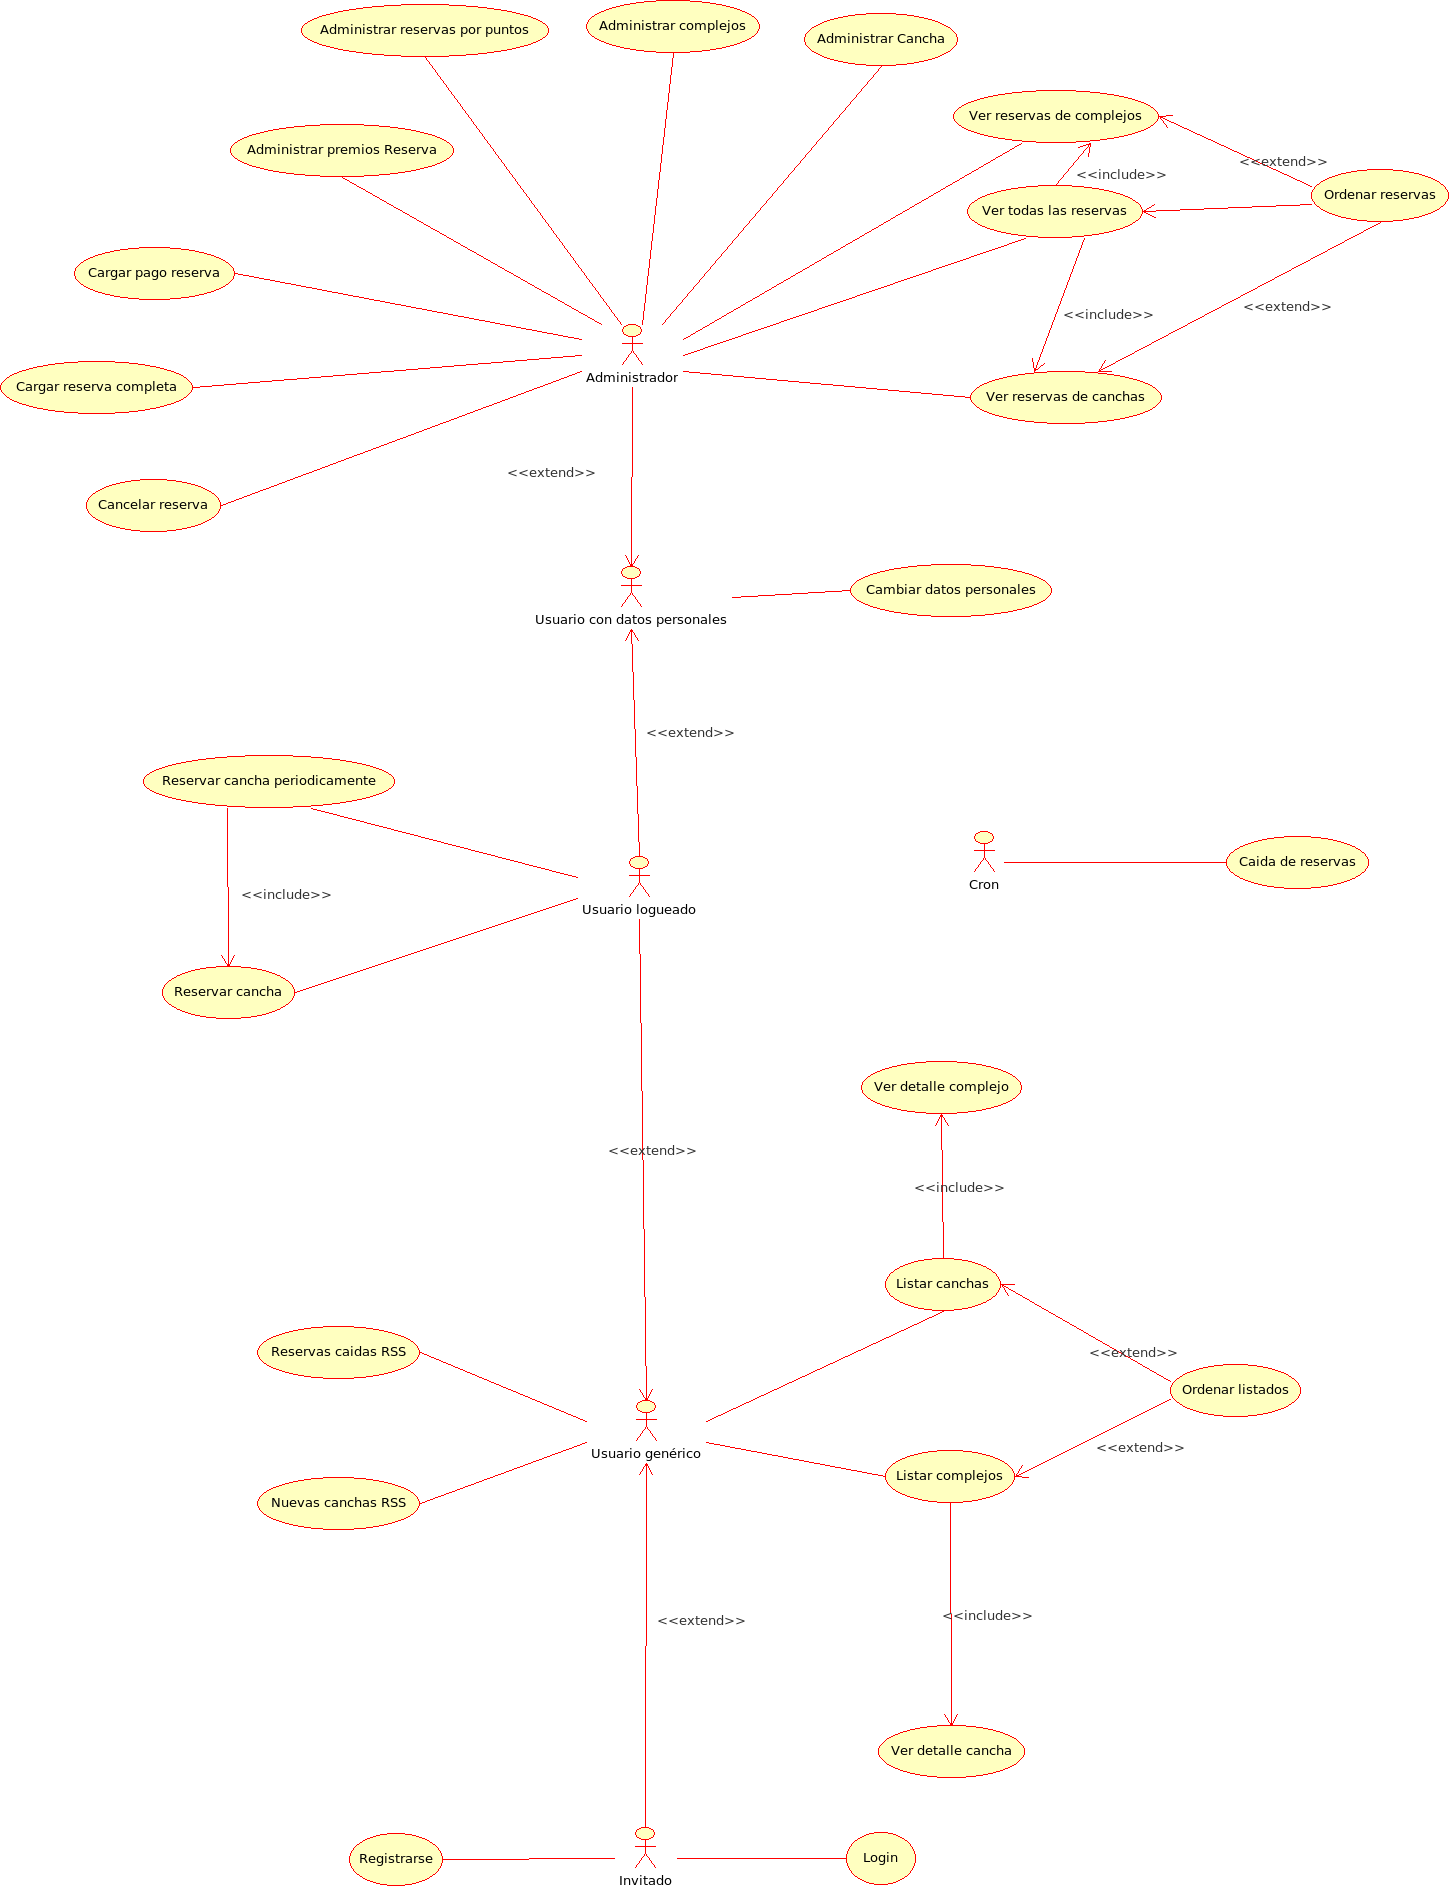
\includegraphics[width=1.00\textwidth]{use_cases.png}
 % use_cases.png: 1449x1890 pixel, 72dpi, 51.12x66.68 cm, bb=0 0 1449 1890
\end{center}

\pagebreak

\section{Casos de Uso}

\subsection{Cambiar datos personales}
\begin{enumerate}

    \item
    \begin{enumerate}
    \item Descripción breve: \\
        Modificación de datos personales de un usuario genérico del sistema.
    \item Actores \\
        Usuario genérico.
    \item Disparadores: \\
        El usuario hace click en \underline{Cambiar datos personales}
        dentro de su panel de usuario.
    \end{enumerate}

    \item Flujo de Eventos:
    \begin{enumerate}

        \item Flujo básico:
            \begin{enumerate}
                \item El usuario hace click en \underline{Cambiar datos personales}.
                \item Luego modifica los datos propios que sean pertinentes a cambiar.
                \item Una vez realizados los cambios hace click en \underline{Guardar}.
            \end{enumerate}
        \item Flujo alternativo:
            \begin{enumerate}
                \item El usuario hace click en \underline{Cambiar datos personales}.
                \item Luego modifica los datos propios que sean pertinentes a cambiar.
                \item Una vez realizados los cambios hace click en \underline{Cancelar}.
            \end{enumerate}
    \end{enumerate}

    \item Precondiciones: \\
        Usuario hizo \underline{Login} como usuario genérico.

    \item Post condiciones \\
        Datos personales del usuario guardados.

\end{enumerate}


% cron caida de reservas
\subsection{Caida de reservas de canchas}
\begin{enumerate}

        \item
	\begin{enumerate}
            \item Descripción breve: \\
                Actualización de las reservas automáticamente cuando alguna reserva
                se da de baja por que se cumplió el tiempo de pago.
            \item Actores \\
                Cron.
            \item Disparadores: \\
                Dada una hora determina se ejecuta automáticamente.
        \end{enumerate}

        \item Flujo de Eventos: 

        \begin{enumerate}
            \item Flujo básico:
                Si existe alguna reserva cuyo tiempo de seña o pago expiró se da de baja.
        \end{enumerate}

        \item Precondiciones: \\
            Reserva existente.

        \item Post condiciones \\
            Reserva dada de baja.

\end{enumerate}


% usuario logueado reservar cancha
\subsection{Reservar cancha}
\begin{enumerate}

    \item
    \begin{enumerate}
    \item Descripción breve: \\
        Este caso de uso describe la reserva de una cancha determinada.
    \item Actores \\
        Usuario genérico.
    \item Disparadores: \\
        El usuario hace click en \underline{Reservar cancha}
        dentro del menu de la cancha.
    \end{enumerate}

    \item Flujo de Eventos: 

    \begin{enumerate}

        \item Flujo básico:
            El usuario hace click en \underline{Reservar cancha}.
            Selecciona el día.
            Selecciona la hora dentro del listado de horarios disponibles
            Hace click en \underline{Reservar}.
    \end{enumerate}

    \item Precondiciones: \\
        Usuario hizo \underline{Login} como usuario genérico.
        La cancha está registrada en el sistema.

    \item Post condiciones \\
        Cancha reservada para el usuario genérico.

\end{enumerate}

% usuario logueado reservar cancha periodicamente
\subsection{Reservar cancha periódicamente}
\begin{enumerate}

    \item
    \begin{enumerate}
    \item Descripción breve: \\
        Este caso de uso describe la reserva periódica de una cancha determinada.
    \item Actores \\
        Usuario genérico.
    \item Disparadores: \\
        El usuario hace click en \underline{Reservar cancha}
        dentro del menu de la cancha.
    \end{enumerate}

    \item Flujo de Eventos:

    \begin{enumerate}

        \item Flujo básico:
            El usuario hace click en \underline{Reservar cancha}.
            Selecciona el día.
            Selecciona la hora dentro del listado de horarios disponibles.
            Selecciona el item \underline{Reservar periódicamente}.
            Hace click en \underline{Reservar}.
    \end{enumerate}

    \item Precondiciones: \\
        Usuario hizo \underline{Login} como usuario genérico.
        La cancha está registrada en el sistema.
        El horario en cuestión no está reservado periódicamente.

    \item Post condiciones \\
        Cancha reservada periódicamente para el usuario genérico.

\end{enumerate}

\subsection{Listar Canchas}
% LISTAR CANCHAS
\begin{enumerate}

    \item
    \begin{enumerate}
    \item Descripción breve: \\
        Se le presenta al usuario un listado de las canchas cargadas en el sistema.
    \item Actores \\
        Usuario genérico.
    \item Disparadores: \\
        El usuario hace click en \emph{Mostrar canchas disponibles}.
    \end{enumerate}

    \item Flujo de Eventos:

    \begin{enumerate}

        \item Flujo básico:
        \begin{enumerate}
            \item El usuario hace click en \emph{Mostrar Canchas Disponibles}
            \item El sistema presenta al usuario un listado de las canchas.
        \end{enumerate}
        \item Flujo alternativo:\\
            No aplica.
        \begin{enumerate}
                    \item El usuario completa algún criterio de ordenación y
                        hace click en \underline{Ordenar Listado}.
        \end{enumerate}
        \begin{enumerate}
                \item El usuario completa algún criterio de filtrado.
                \item El sistema refresca el listado siguiendo el criterio de filtrado.
        \end{enumerate}
    \end{enumerate}

    \item Precondiciones: \\
        No aplica.

    \item Post condiciones \\
        Listado de canchas presentado al usuario.

\end{enumerate}

\subsection{Listar Complejos}
% LISTAR COMLEJOS
\begin{enumerate}

    \item
    \begin{enumerate}
    \item Descripción breve: \\
        Se le presenta al usuario un listado de las complejos deportivos cargados en el sistema.
    \item Actores \\
        Usuario genérico.
    \item Disparadores: \\
        El usuario hace click en \emph{Mostrar Complejos}.
    \end{enumerate}

    \item Flujo de Eventos: 

    \begin{enumerate}

        \item Flujo básico:
        \begin{enumerate}
            \item El usuario hace click en \emph{Mostrar Complejos}
            \item El sistema presenta al usuario un listado de los complejos.
        \end{enumerate}
        \item Flujo alternativo:\\
        \begin{enumerate}
            \item El usuario completa algún criterio de ordenación y
                hace click en \underline{Ordenar Listado}.
        \end{enumerate}
        \begin{enumerate}
            \item El usuario completa algún criterio de filtrado.
            \item El sistema refresca el listado siguiendo el criterio de filtrado.
        \end{enumerate}
    \end{enumerate}

    \item Precondiciones: \\
        No aplica.

    \item Post condiciones \\
        Listado de complejos presentado al usuario.

\end{enumerate}

\subsection{Ordenar Listados}
% ORDENAR LISTADO
\begin{enumerate}

    \item
    \begin{enumerate}
    \item Descripción breve: \\
        Se le permite al usuario ordenar un listado siguiendo diversos criterios.
    \item Actores \\
        Usuario genérico.
    \item Disparadores: \\
        El usuario hace click en \emph{Ordenar Listado}.
    \end{enumerate}

    \item Flujo de Eventos: 

    \begin{enumerate}

        \item Flujo básico:
        \begin{enumerate}
                    \item El usuario selecciona el criterio de ordenación.
                    \item El usuario hace click en \emph{Ordenar Listado}.
        \end{enumerate}
        \item Flujo alternativo:\\

    \end{enumerate}

    \item Precondiciones: \\
        Listado cargado previamente.

    \item Post condiciones \\
        Listado ordenado según criterio seleccionado.

\end{enumerate}

% VER DETALLE CANCHA

\subsection{Ver detalle complejo}
\begin{enumerate}

    \item
    \begin{enumerate}
    \item Descripción breve: \\
        Se muestra en detalle las características de una cancha.
    \item Actores \\
        Administrador.
    \item Disparadores: \\
        Click en el botón \emph{Ver detalles} dentro de la
        página que lista las canchas o en la vista dellada de un complejo.
    \end{enumerate}

    \item Flujo de Eventos: 

    \begin{enumerate}

        \item Flujo básico:
        \begin{enumerate}
            \item El usuario selecciona \underline{Listar Canchas Disponibles}
                o \underline{Ver detalles} en el listado de complejos.
            \item El usuario hace click en \underline{Ver detalles}
            \item Se le presenta al usuario informacion detallada sobre la cancha seleccionada.
        \end{enumerate}
    \item Flujo alternativo:\\
    \end{enumerate}

    \item Precondiciones: \\
        Usuario logueado como usuario común.

    \item Post condiciones \\
        Detalles de la cancha presentados al usuario.

\end{enumerate}

% ADMINISTRAR COMPLEJOS
\subsection{Administrar complejos}
\begin{enumerate}

    \item
    \begin{enumerate}
    \item Descripción breve: \\
        Este caso de uso describe las operaciones de creación, borrado y
        modificación de complejos.
    \item Actores \\
        Administrador.
    \item Disparadores: \\
        El administrador selecciona las operaciones explícitamente de su panel
        de administración.
    \end{enumerate}

    \item Flujo de Eventos: 

    \begin{enumerate}

        \item Flujo básico:
            El usuario selecciona \underline{Listar complejos}.
        \item Flujos alternativos:\\
            \begin{enumerate}
                \item \underline{Crear complejo} \\
                \begin{enumerate}
                    \item El usuario hace click en \textit{Crear nuevo complejo}
                    en el panel de administración.
                    \item El usuario completa los datos solicitados: País, 
                    provincia, localidad y barrio; teléfono, dirección, horario 
                    general de atención.
                    Se pueden indicar en forma opcional los rangos de puntos con
                    el vencimiento de los distintos estados de las canchas, el 
                    precio de las canchas y el porcentaje que corresponde a la
                    reserva.
                    \item El usuario da por finalizada la creación haciendo click
                    en \textit{Guardar complejo}.
                \end{enumerate}
                \item \underline{Modificar complejo} \\
                \begin{enumerate}
                    \item El usuario hace click en \textit{Modificar complejo} 
                    dentro de la entrada del listado que corresponde al complejo 
                    que desea modificar.
                    \item El usuario modifica los datos deseados.
                    \item El usuario da por finalizada la modificación haciendo 
                    click en \textit{Guardar complejo}.
                \end{enumerate}
                \item \underline{Borrar complejo}
                \begin{enumerate}
                    \item El usuario hace click en \textit{Borrar complejo}
                    dentro de la entrada del listado que corresponde al complejo
                     que desea eliminar.
                    \item El usuario confirma que desea eliminar el elemento
                    seleccionado.
                \end{enumerate}
            \end{enumerate}
    \end{enumerate}

    \item Precondiciones: \\
        Usuario hizo \underline{Login} como administrador.

    \item Post condiciones \\
        No aplica.

\end{enumerate}

% ADMINISTRAR CANCHAS

\subsection{Administrar canchas}
\begin{enumerate}

    \item
    \begin{enumerate}
    \item Descripción breve: \\
        Este caso de uso describe las operaciones de creación, borrado y
        modificación de canchas.
    \item Actores \\
        Administrador.
    \item Disparadores: \\
        El administrador selecciona las operaciones explícitamente de la página
        de administración de un complejo existente.
    \end{enumerate}

    \item Flujo de Eventos: 

    \begin{enumerate}

        \item Flujo básico:
            El usuario selecciona un complejo a través de 
            \underline{Listar complejos} y luego hace click en 
            \underline{Listar canchas}.
        \item Flujos alternativos:\\
            \begin{enumerate}
                \item \underline{Crear cancha} \\
                \begin{enumerate}
                    \item El usuario hace click en \textit{Crear nueva cancha}
                    en el listado de canchas del complejo elegido.
                    \item El usuario indica la cantidad de jugadores, el tipo de
                    piso y si la cancha es o no techada.
                    \item El usuario da por finalizada la creación haciendo click
                    en \textit{Guardar cancha}.
                \end{enumerate}
                \item \underline{Modificar cancha} \\
                \begin{enumerate}
                    \item El usuario hace click en \textit{Modificar cancha} 
                    dentro de la entrada del listado que corresponde a la cancha 
                    que desea modificar.
                    \item El usuario modifica los datos deseados.
                    \item El usuario da por finalizada la modificación haciendo 
                    click en \textit{Guardar cancha}.
                \end{enumerate}
                \item \underline{Borrar cancha}
                \begin{enumerate}
                    \item El usuario hace click en \textit{Borrar cancha}
                    dentro de la entrada del listado que corresponde a la cancha
                     que desea eliminar.
                    \item El usuario confirma que desea eliminar el elemento
                    seleccionado.
                \end{enumerate}
            \end{enumerate}
    \end{enumerate}

    \item Precondiciones: \\
        Usuario hizo \underline{Login} como administrador.

    \item Post condiciones \\
        No aplica.

\end{enumerate}

% ADMINISTRAR PREMIOS POR RESERVAS

\subsection{Administrar premios por reservas}
\begin{enumerate}

    \item
    \begin{enumerate}
    \item Descripción breve: \\
        Este caso de uso describe como se define la cantidad de puntos que gana
        un usuario al pasar por los distintos estados de una reserva, de acuerdo
        al sistema de puntos.
    \item Actores \\
        Administrador.
    \item Disparadores: \\
        El administrador hace click en \underline{Administrar premios por reserva}
        dentro de su panel de administración.
    \end{enumerate}

    \item Flujo de Eventos: 

    \begin{enumerate}

        \item Flujo básico:
            El usuario hace click en \underline{Administrar premios por reserva}.
            Luego determina cuantos puntos se otorgarán para las acciones de
            \textit{Reservar}, \textit{Señar} y \textit{Pagar}.
            También debe indicar cuántos puntos pierde el usuario si se cae
            su reserva, según ya estuviese reservada o señada.
    \end{enumerate}

    \item Precondiciones: \\
        Usuario hizo \underline{Login} como administrador.

    \item Post condiciones \\
        Todas las acciones tienen un puntaje asociado. Sistema de puntos
        actualizado.

\end{enumerate}

% ADMINISTRAR LIMITES DE RESERVAS POR PUNTOS

\subsection{Administrar límites de reservas por puntos}
\begin{enumerate}

    \item
    \begin{enumerate}
    \item Descripción breve: \\
        Este caso de uso describe como se definen los plazos de vencimiento de
        las reservas según el puntaje del usuario que haya realizado la reserva.
    \item Actores \\
        Administrador.
    \item Disparadores: \\
        El administrador hace click en 
        \underline{Administrar límites de reserva por puntos}
        dentro de su panel de administración.
    \end{enumerate}

    \item Flujo de Eventos: 

    \begin{enumerate}

        \item Flujo básico:
            El usuario hace click en \underline{Administrar límites de reserva
            por puntos}.
            Luego se determina cuales serán los plazos máximos de tiempo para la
            caducidad de cada complejo y cada cancha, teniendo en cuenta el rango
            de puntos que tenga el usuario.
    \end{enumerate}

    \item Precondiciones: \\
        Usuario hizo \underline{Login} como administrador.

    \item Post condiciones \\
        No aplica.

\end{enumerate}


\subsection{RSS: Ver reservas caidas}
% reservas caidas rss
\begin{enumerate}

    \item
        \begin{enumerate}
            \item Descripción breve: \\
                Se listan los complejos con las últimas reservas caidas.
            \item Actores \\
                Usuario genérico, invitado.

            \item Disparadores: \\
                Acceso a la url del \emph{RSS} de reservas caidas.

        \end{enumerate}

    \item Flujo de Eventos:

        \begin{enumerate}
            \item Flujo básico:
                Un usuario genérico accede a la url del \emph{RSS}  de reservas caidas
                y visualiza el listado de reservas que fueron dadas de baja. El listado
                contiene la información necesaria como para que el lector del \emph{RSS}
                pueda realizar una nueva reserva.
        \end{enumerate}

    \item Precondiciones: \\
        No aplica.

    \item Post condiciones \\
        No aplica.

\end{enumerate}

% nuevas canchas rss
\subsection{RSS: Ver nuevas canchas}
\begin{enumerate}

    \item
    \begin{enumerate}
        \item Descripción breve: \\
            Se listan las últimas canchas agregadas al sistema.
        \item Actores \\
            Usuario genérico, invitado.
        \item Disparadores: \\
            Acceso a la url del \emph{RSS} de canchas nuevas.

    \end{enumerate}

    \item Flujo de Eventos: 

        \begin{enumerate}
            \item Flujo básico:
                Un usuario genérico accede a la url del \emph{RSS}  de canchas nuevas
                y visualiza el listado de canchas que fueron agregadas al sistema. El
                listado contiene información sobre el complejo y barrio para facilitar
                al lector del \emph{RSS} la reserva de la cancha.
        \end{enumerate}

    \item Precondiciones: \\
        El lector del \emph{RSS} no necesita estar logueado como usuario.

    \item Post condiciones \\
        No aplica.

\end{enumerate}

% invitado registrarse
\subsection{Invitado registrarse}
\begin{enumerate}

    \item
        \begin{enumerate}
            \item Descripción breve: \\
                Obtener una cuenta de usuario del sistema.
            \item Actores \\
                Invitado.
            \item Disparadores: \\
                Click en \underline{registrarse} en la pantalla principal del sistema.

        \end{enumerate}

    \item Flujo de Eventos:

        \begin{enumerate}
            \item Flujo básico:
                Un usuario genérico accede a la pantalla principal del sistema y
                hace click en \underline{registrarse}. Ingresa los datos necesarios
                para registrarse como usuario del sistema.

            \item Flujo alternativo:\\
                Se muestra un cartel que informa que los datos ingresados son
                incorrectos, puede volver a intentarlo.

                \begin{enumerate}
                    \item Condición 1 \\
                            El usuario ingresado ya existe dentro del sistema.
                    \item Condición 2 \\
                            Faltan datos requeridos.
                    \item Condición 3 \\
                            Las contrase\~nas ingresadas no son iguales.
                    \item Condición 4 \\
                            Alguna combinación de las anteriores.
                \end{enumerate}
	\end{enumerate}

    \item Precondiciones: \\
        No debe estar registrado como usuario del sistema.

    \item Post condiciones \\
        El invitado obtiene una cuenta de usuario del sistema.

\end{enumerate}

% invitado login
\subsection{Invitado login}
\begin{enumerate}

    \item
        \begin{enumerate}
            \item Descripción breve: \\
                Acceso al sistema como usuario.
            \item Actores \\
                Usuario del sistema.
            \item Disparadores: \\
                Acceso a la pantalla principal del sistema.
        \end{enumerate}

    \item Flujo de Eventos:
        \begin{enumerate}
            \item Flujo básico:
                Un usuario genérico accede a la pantalla principal del sistema.
                Ingresa nombre de usuario, tipo y contraseña. Si los datos son
                válidos, tiene acceso al sistema.

            \item Flujo alternativo:\\
                Se muestra un cartel que informa que los datos ingresados son
                incorrectos, puede volver a intentarlo.

                \begin{enumerate}
                \item Condición 1 \\
                    El usuario ingresado es incorrecto.
                \item Condición 2 \\
                    El tipo de usuario ingresado es incorrecto.
                \item Condición 3 \\
                    La contraseña ingresada es incorrecta.
                \item Condición 4 \\
                    Alguna combinación de las anteriores.
                \end{enumerate}

        \end{enumerate}

        \item Precondiciones: \\
            Debe estar registrado como usuario del sistema.

        \item Post condiciones \\
            El usuario tiene acceso al sistema.

\end{enumerate}

\subsection{Cargar pago reservas}
\begin{enumerate}

    \item
    \begin{enumerate}
    \item Descripción breve: \\
        Se carga un pago para una determinada reserva.
    \item Actores \\
        Administrador.
    \item Disparadores: \\
        Click en el botón \underline{Cargar pago de reserva} dentro de la
        página que muestra las reservas para una cancha.
    \end{enumerate}

    \item Flujo de Eventos: 

    \begin{enumerate}

        \item Flujo básico:
            Un usuario genérico hace \underline{Login} como administrador y
            hace click en \underline{Ver reservas de canchas}. Luego para una
            reserva particular hace click en
            \underline{Cargar pago de reserva}. El administrador ingresa el
            monto que fue pagado de la reserva. En el caso de que se logre el
            mínimo para pasar a estado señada se pasa la reserva a dicho
            estado, lo mismo si se completa el pago total, pasándola a estado
            pagada; en ambos casos se actualizan los puntos del usuario que
            emitió la reserva y se informa al usuario que la operación fue
            exitosa. En caso contrario, ya que la cantidad ingresada es
            incorrecta, se procede al \underline{Flujo alternativo 1}.


        \item Flujos alternativos:\\
            Se muestra un cartel que informa que la cantidad ingresada es
            incorrecta.
            \begin{enumerate}
                \item Condición 1 \\
                    La cantidad ingresada es incorrecta.
            \end{enumerate}

    \end{enumerate}

    \item Precondiciones: \\
        Ususario logueado como administrador.

    \item Post condiciones \\
        Pago de la reserva cargado y, si aplica, estado de la reserva y puntos
        del usuario que emitió la reserva actualizados.

\end{enumerate}

\subsection{Cargar reserva completa}
\begin{enumerate}

    \item
    \begin{enumerate}
    \item Descripción breve: \\
        Se carga un pago completo para una determinada reserva.
    \item Actores \\
        Administrador.
    \item Disparadores: \\
        Click en el botón \underline{Cargar pago completo de reserva} dentro
        de la página que muestra las reservas para una cancha.
    \end{enumerate}

    \item Flujo de Eventos:

    \begin{enumerate}

        \item Flujo básico:
            Un usuario genérico hace \underline{Login} como administrador y
            hace click en \underline{Ver reservas de canchas}. Luego para una
            reserva particular hace click en
            \underline{Cargar pago completo de reserva}. La reserva pasa al
            estado pagada y se actualizan los puntos del usuario que emitió la
            reserva. Se informa al usuario que la operación fue exitosa.

    \end{enumerate}

    \item Precondiciones: \\
        Ususario logueado como administrador.

    \item Post condiciones \\
        Pago de la reserva cargado y estado de la reserva actualizado a pagada.
        Puntos del usuario que emitió la reserva actualizados.

\end{enumerate}

\subsection{Cancelar reserva}
\begin{enumerate}

    \item
    \begin{enumerate}
    \item Descripción breve: \\
        Se da de baja una determinada reserva.
    \item Actores \\
        Usuario logueado como usuario común.
    \item Disparadores: \\
        Click en el botón \underline{Cancelar reserva} dentro de la
        página que muestra las reservas de una cancha.
    \end{enumerate}

    \item Flujo de Eventos:

    \begin{enumerate}

        \item Flujo básico:
            Un usuario genérico hace \underline{Login} como usuario común y
            hace click en \underline{Ver reservas de canchas}. Luego para una
            reserva particular hace click en \underline{Cancelar reserva}.
            La reserva se elimina del sistema. Se informa al usuario que la
            operación fue exitosa.

    \end{enumerate}

    \item Precondiciones: \\
        Ususario logueado como usuario común.

    \item Post condiciones \\
        Reserva dada de baja.

\end{enumerate}

\subsection{Ver detalle complejo}
\begin{enumerate}

    \item
    \begin{enumerate}
    \item Descripción breve: \\
        Se muestra en detalle las características de un complejo.
    \item Actores \\
        Administrador.
    \item Disparadores: \\
        Click en el botón \underline{Ver detalle} dentro de la
        página que lista los complejos del sistema.
    \end{enumerate}

    \item Flujo de Eventos:

    \begin{enumerate}

        \item Flujo básico:
            Un usuario genérico hace \underline{Login} como usuario común y
            hace click en \underline{Listar complejos}. Se visualiza el
            complejo seleccionado, las canchas que tiene, la información del
            mismo y todos los datos que contiene. A su vez tiene el detalle de
            cada cancha, el cual consiste de sus características y los horarios
            disponibles en un calendario.


    \end{enumerate}

    \item Precondiciones: \\
        Usuario logueado como usuario común.

    \item Post condiciones \\
        No aplica.

\end{enumerate}

\subsection{Ver todas las reservas}
\begin{enumerate}

    \item
    \begin{enumerate}
    \item Descripción breve: \\
        Se listan todas las reservas existentes.
    \item Actores \\
        Administrador.
    \item Disparadores: \\
        Click en el botón \underline{Ver reservas} dentro de la
        página principal del administrador.
    \end{enumerate}

    \item Flujo de Eventos: 

    \begin{enumerate}

        \item Flujo básico:
            Un Administrador hace click en \underline{Ver reservas}.
        \item Flujos alternativos:\\
            Se muestra un cartel que no existen reservas.
            \begin{enumerate}
                \item Condición 1 \\
                    No existen reservas de ningún tipo.
            \end{enumerate}

    \end{enumerate}

    \item Precondiciones: \\
        Administrador logueado como administrador.

    \item Post condiciones \\
        No aplica.

\end{enumerate}

\subsection{Ver reservas de canchas}
\begin{enumerate}

    \item
    \begin{enumerate}
    \item Descripción breve: \\
        Se listan las reservas de canchas.
    \item Actores \\
        Administrador.
    \item Disparadores: \\
        Click en el botón \underline{Ver reservas de canchas}
        dentro de la página principal del administrador.
    \end{enumerate}

    \item Flujo de Eventos:

    \begin{enumerate}

        \item Flujo básico:
            Un Administrador hace click en \underline{Ver reservas} y luego
            en \underline{Ver reservas de canchas}.
        \item Flujos alternativos:\\
            Se muestra un cartel que no existen reservas de cancha.
            \begin{enumerate}
                \item Condición 1 \\
                    No existen reservas de canchas.
            \end{enumerate}

    \end{enumerate}

    \item Precondiciones: \\
        Administrador logueado como administrador.

    \item Post condiciones \\
        No aplica.

\end{enumerate}

\subsection{Ver reservas de complejos}
\begin{enumerate}

    \item
    \begin{enumerate}
    \item Descripción breve: \\
        Se listan las reservas de complejos.
    \item Actores \\
        Administrador.
    \item Disparadores: \\
        Click en el botón \underline{Ver reservas de complejos}
        dentro de la página principal del administrador.
    \end{enumerate}

    \item Flujo de Eventos:

    \begin{enumerate}

        \item Flujo básico:
            Un Administrador hace click en \underline{Ver reservas} y luego
            en \underline{Ver reservas de complejos}.
        \item Flujos alternativos:\\
            Se muestra un cartel que no existen reservas de complejos.
            \begin{enumerate}
                \item Condición 1 \\
                    No existen reservas de complejos.
            \end{enumerate}

    \end{enumerate}

    \item Precondiciones: \\
        Administrador logueado como administrador.

    \item Post condiciones \\
        No aplica.

\end{enumerate}

\subsection{Ordenar reservas}
\begin{enumerate}

    \item
    \begin{enumerate}
    \item Descripción breve: \\
        Se ordenan los listados de reservas.
    \item Actores \\
        Administrador.
    \item Disparadores: \\
        Click en el botón \underline{Ordenar reservas}
        dentro de cualquier listado de reservas.
    \end{enumerate}

    \item Flujo de Eventos: 

    \begin{enumerate}

        \item Flujo básico:
            Un Administrador hace click en \underline{Ver reservas} y luego
            en \underline{Ordenar reservas}.
        \item Flujos alternativos:\\
            No aplica.
    \end{enumerate}

    \item Precondiciones: \\
        \begin{enumerate}
            \item Administrador logueado como administrador.
            \item Existencia de reservas.
        \end{enumerate}

    \item Post condiciones \\
        No aplica.

\end{enumerate}

\end{document}
